\begin{figure}[ht!]
\centering
% manually adjust the width of the figure
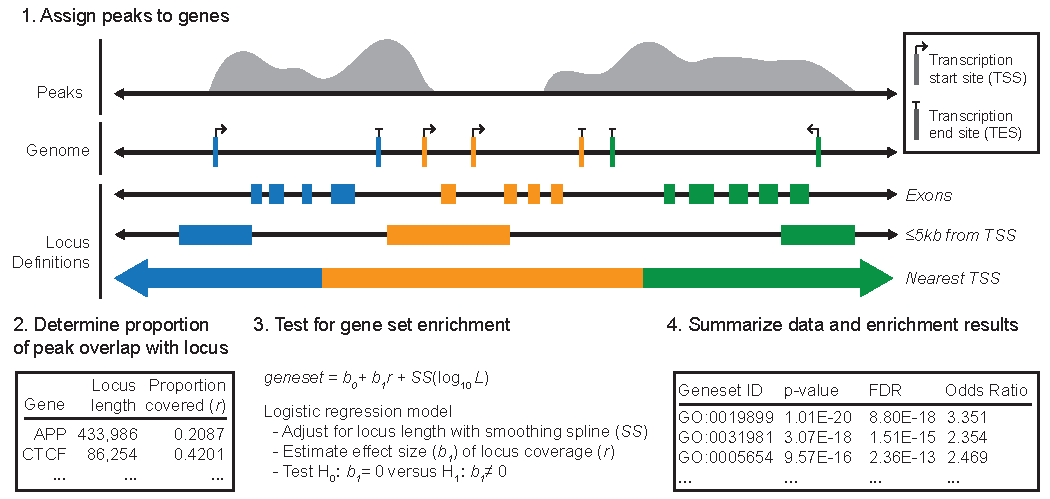
\includegraphics[width=1\textwidth]{chap2figs/figure2_1.pdf}
\caption[Broad-Enrich functions in four steps.]
{
% Rackham requires the figure list title matches the first sentence, so repeat that sentence here
\textbf{Broad-Enrich functions in four steps.}
(1) The user selects a gene locus definition (exons, $\leq$ 5kb, and nearest TSS are shown). (2) The proportion of each gene locus covered by ChIP-seq peaks from a given HM, or otherwise derived genomic regions, is determined. (3) For each gene set to be tested, logistic regression is performed using the model shown, where geneset refers to the binary vector of gene set membership, r refers to the vector of proportions of the gene loci covered by all peaks overlapping the respective loci, SS is a binomial cubic smoothing spline which corrects for any locus length bias, and L is a vector of gene locus lengths. (4) P-values for enrichment or depletion are adjusted for multiple testing and users are provided summarized functional enrichment results, peak to gene loci assignments, and diagnostic plots.
}
\label{chap2:fig:1}
\end{figure}

\newpage

\begin{figure}[ht!]
\centering
% manually adjust the width of the figure
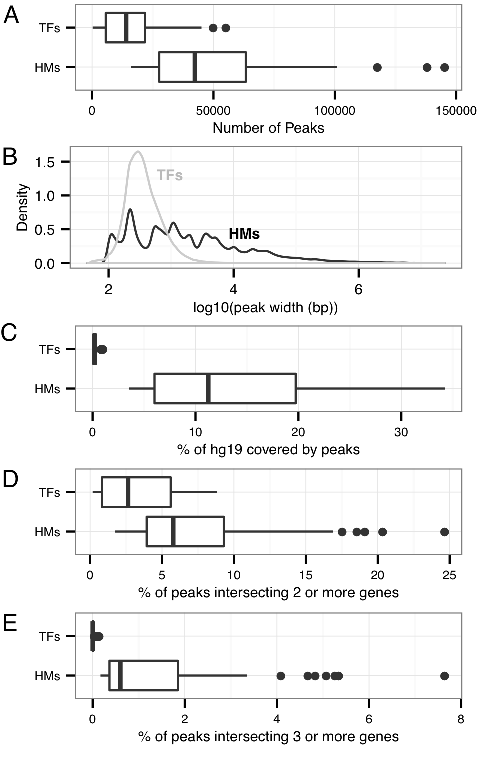
\includegraphics[width=0.7\textwidth]{chap2figs/figure2_2.pdf}
\caption[Histone (HM) and transcription-factor (TF) based peak sets exhibit several different properties.]
{
% Rackham requires the figure list title matches the first sentence, so repeat that sentence here
\textbf{Histone (HM) and transcription-factor (TF) based peak sets exhibit several different properties.} Observed over 100 TF and 55 HM ENCODE ChIP-seq datasets. (A) There tends to be more peaks in HM  experiments (median = 42,330) compared to TF experiments (median = 14,040). (B) The peak width distributions are significantly different. HM peaks (black) tend to be broad and highly variable (median = 1,255 bp, sd = 483,279 bp), while TF peaks (gray) tend to be narrow and less variable (median = 330 bp, sd = 560 bp). (C) HM peaks consistently cover a greater percentage of hg19 (median = 11.25\%) than TF peaks (median = 0.16\%). (D) The percentage of peaks covering two or more gene loci also tends to be higher for HMs (median = 5.78\%) than for TFs (median = 2.64\%). (E) The same is true of peaks covering three or more gene loci (median = 0.6\% and 0\%, respectively). Both (D) and (E) use the nearest TSS definition.
}
\label{chap2:fig:2}
\end{figure}

\newpage

\begin{figure}[ht!]
\centering
% manually adjust the width of the figure
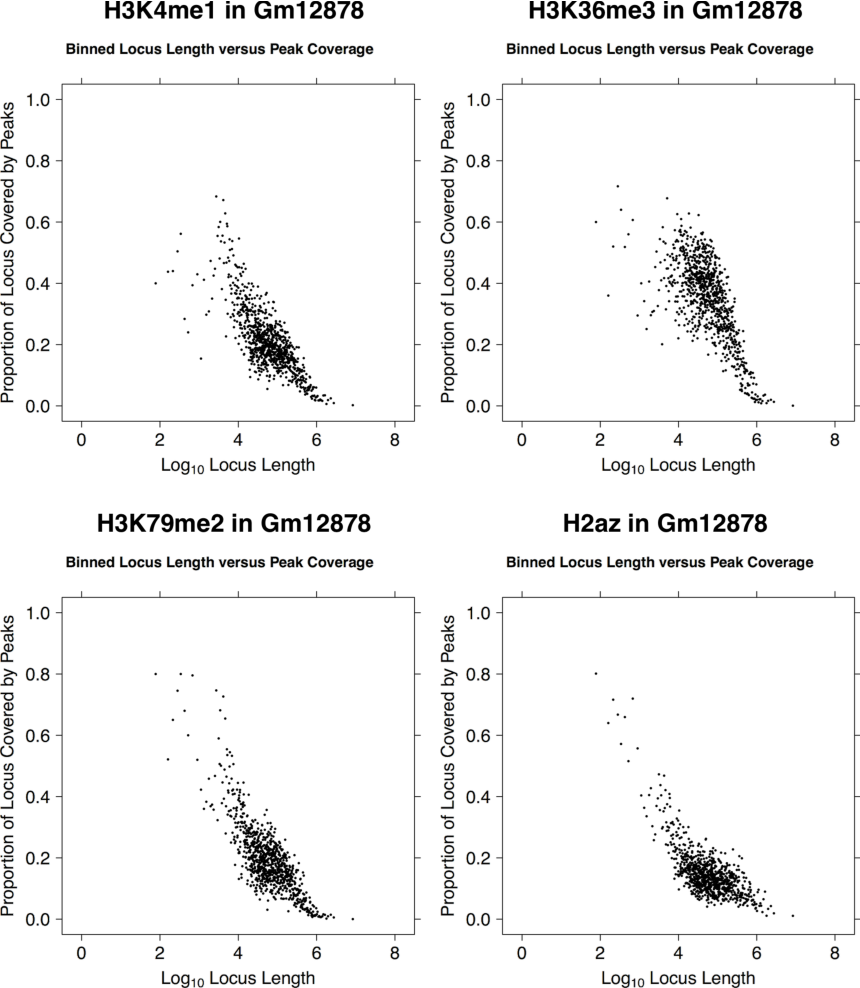
\includegraphics[width=0.7\textwidth]{chap2figs/figure2_3.pdf}
\caption[The relationship between gene locus length and the percentage of the locus covered by a peak.]
{
% Rackham requires the figure list title matches the first sentence, so repeat that sentence here
\textbf{The relationship between gene locus length and the percentage of the locus covered by a peak.} For selected HM datasets in cell line GM12878 using the nearest TSS locus definition. For visualization purposes, genes were binned in groups of 25 by their locus length, such that each point represents the average of 25 genes. There tends to be a strong negative correlation between log10 locus length and the proportion of the locus covered by a peak.
}
\label{chap2:fig:3}
\end{figure}

\newpage

\begin{figure}[ht!]
\centering
% manually adjust the width of the figure
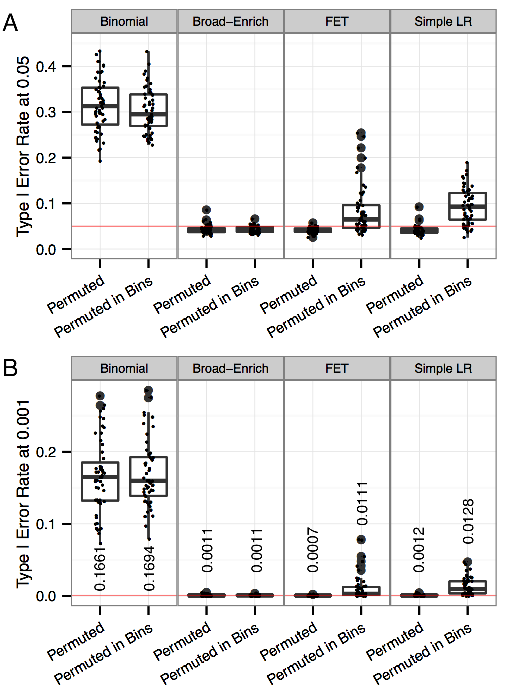
\includegraphics[width=0.7\textwidth]{chap2figs/figure2_4.pdf}
\caption[Type I error rates for enrichment tests.]
{
% Rackham requires the figure list title matches the first sentence, so repeat that sentence here
\textbf{Type I error rates for enrichment tests.} Type I error rates of the binomial-based test, Broad-Enrich, the simple LR model, and Fisher's exact test under the two permutation scenarios with the nearest TSS locus definition. Each point represents 1 of the 55 HM datasets. (A) At $\alpha = 0.05$  (red line), we find inflated type I error for the binomial test under both permutation scenarios, the correct error rate for Broad-Enrich, and the correct error rate for permutations eliminating length bias but often inflated error for permutations preserving length bias for both the simple LR model and Fisher's exact test. (B) At $\alpha = 0.001$ (red line), we observe results similar to $\alpha = 0.05$. Mean error rates are given inset.
}
\label{chap2:fig:4}
\end{figure}

\newpage

\begin{figure}[ht!]
\centering
% manually adjust the width of the figure
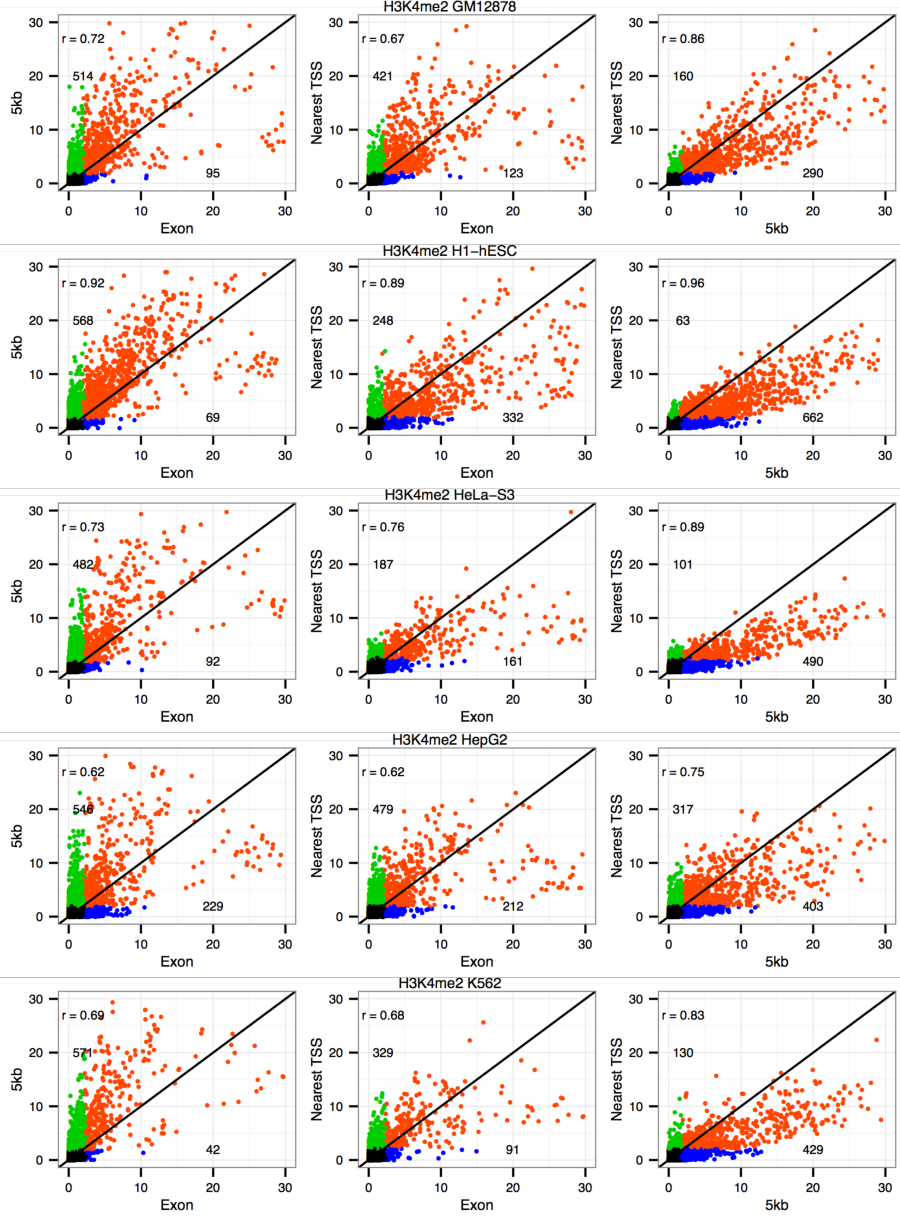
\includegraphics[width=0.8\textwidth]{chap2figs/figure2_5.pdf}
\caption[H3K4me2 enrichment signal for different locus definitions.]
{
% Rackham requires the figure list title matches the first sentence, so repeat that sentence here
\textbf{H3K4me2 enrichment signal for different locus definitions.} Enrichment signal (-log10 p-value) comparing nearest TSS, $\leq$ 5kb from TSS, and exons locus definitions for H3K4me2 across 5 cell lines. H3K4me2 tends to occur in the proximal promoter, and $\leq$ 5kb tends to perform better versus nearest TSS and versus exons. Axes limits are constrained for visual clarity. Pearson correlation coefficient of all p-values (including those outside axis limits) is reported inset. Green points are unique enrichments ($\beta_1 > 0$ and $FDR < 0.05$) for the locus definition on the y-axis (number is inset), blue points are unique enrichments for the locus definitions on the x-axis (number is inset), orange points are enriched in both, and black in neither.
}
\label{chap2:fig:5}
\end{figure}

\newpage

\begin{figure}[ht!]
\centering
% manually adjust the width of the figure
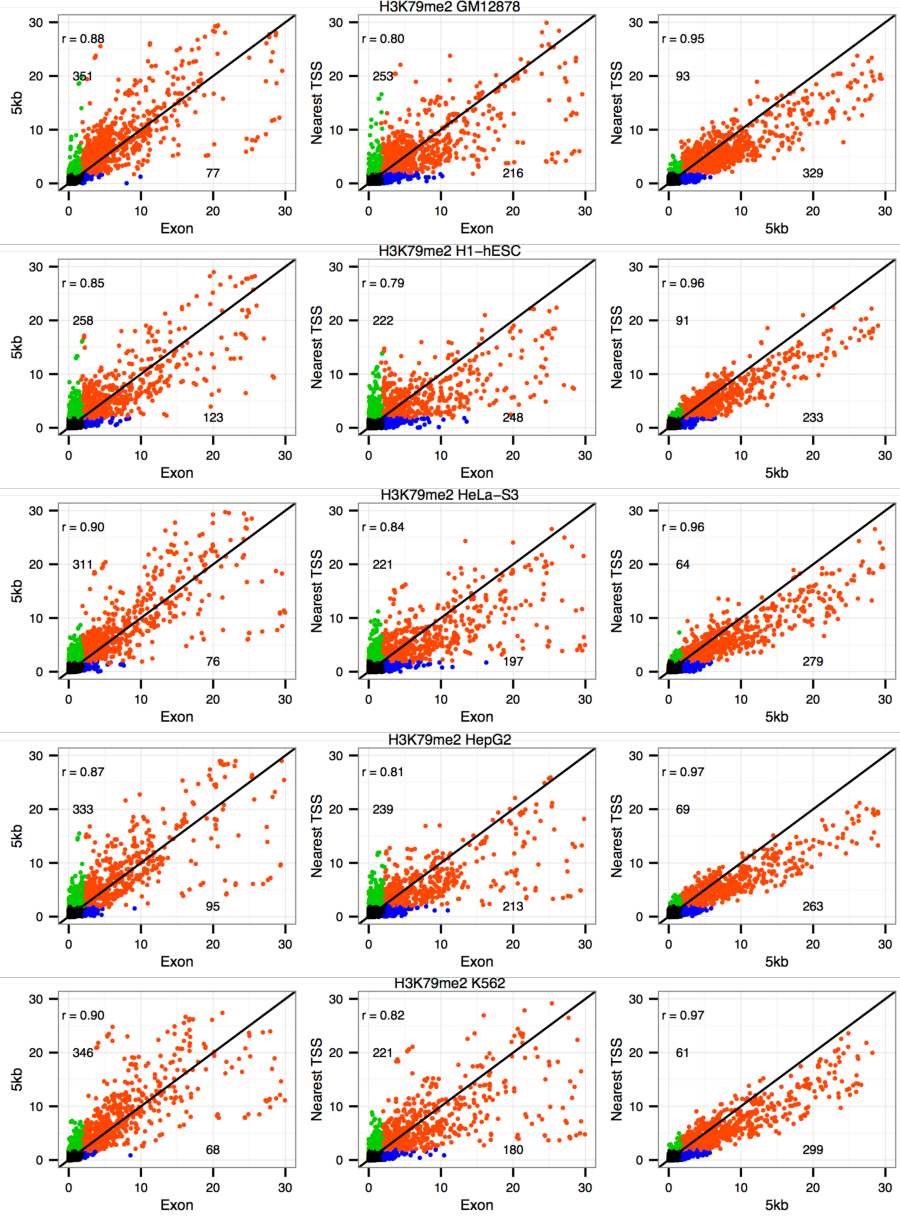
\includegraphics[width=0.8\textwidth]{chap2figs/figure2_6.pdf}
\caption[H3K79me2 enrichment signal for different locus definitions.]
{
% Rackham requires the figure list title matches the first sentence, so repeat that sentence here
\textbf{H3K79me2 enrichment signal for different locus definitions.} Enrichment signal (-log10 p-value) comparing nearest TSS, $\leq$ 5kb from TSS, and exons locus definitions for H3K79me2 across 5 cell lines. H3K79me2 preferentially occurs at the 5' end of genes, which is best captured by the $\leq$ 5kb locus definition, and $\leq$ 5kb performs better versus both nearest TSS and exons. Axes limits are constrained for visual clarity. Pearson correlation coefficient of all p-values (including those outside axis limits) is reported inset. Green points are unique enrichments ($\beta_1 > 0$ and $FDR < 0.05$) for the locus definition on the y-axis (number is inset), blue points are unique enrichments for the locus definitions on the x-axis (number is inset), orange points are enriched in both, and black in neither.
}
\label{chap2:fig:6}
\end{figure}

\newpage

\begin{figure}[ht!]
\centering
% manually adjust the width of the figure
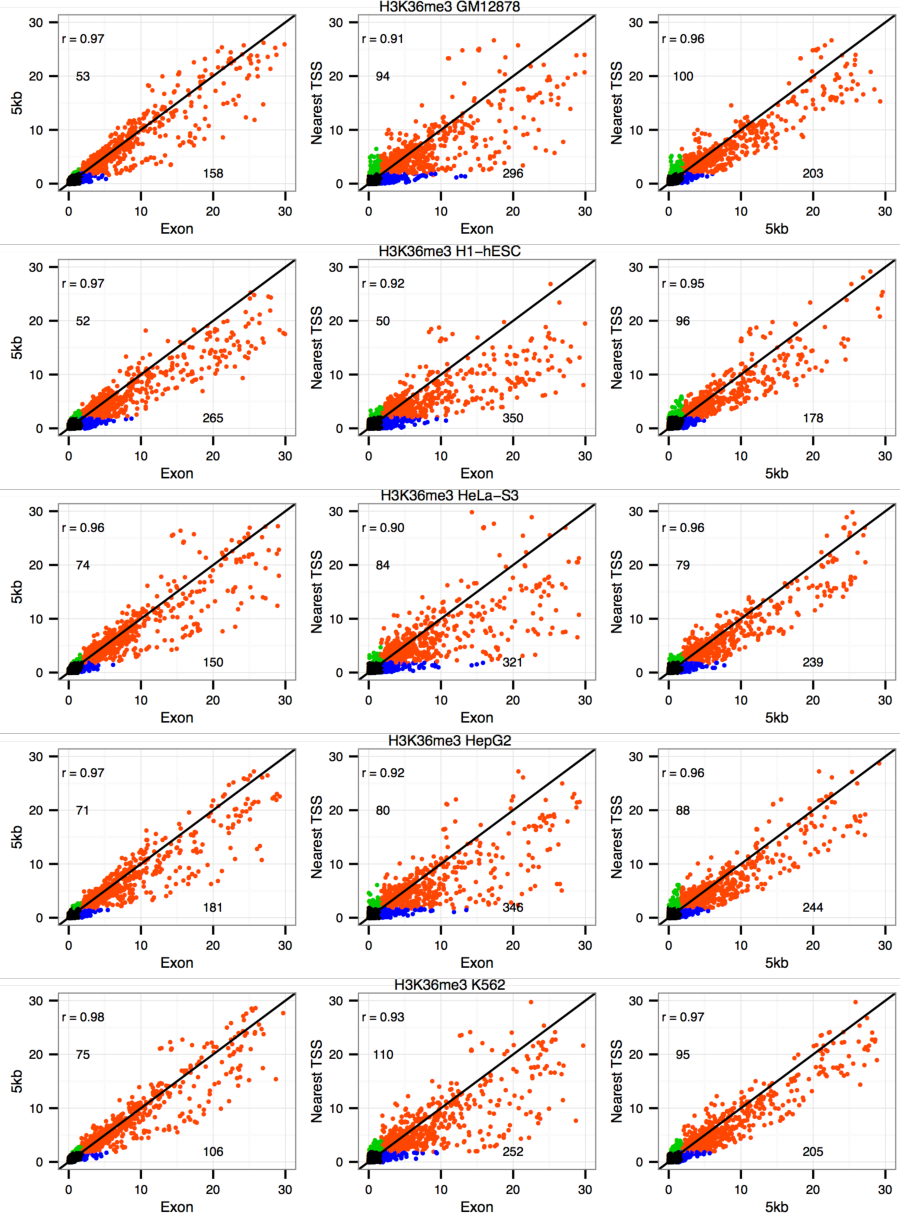
\includegraphics[width=0.8\textwidth]{chap2figs/figure2_7.pdf}
\caption[H3K36me3 enrichment signal for different locus definitions.]
{
% Rackham requires the figure list title matches the first sentence, so repeat that sentence here
\textbf{H3K36me3 enrichment signal for different locus definitions.} Enrichment signal (-log10 p-value) comparing nearest TSS, $\leq$ 5kb from TSS, and exons locus definitions for H3K36me3 across 5 cell lines. H3K36me3 preferentially occurs near the 3' end of genes, perhaps out of reach of the $\leq$ 5kb locus definition. The exons definition tends to provide stronger enrichment signal versus both nearest TSS and $\leq$ 5kb. Axes limits are constrained for visual clarity. Pearson correlation coefficient of all p-values (including those outside axis limits) is reported inset. Green points are unique enrichments ($\beta_1 > 0$ and $FDR < 0.05$) for the locus definition on the y-axis (number is inset), blue points are unique enrichments for the locus definitions on the x-axis (number is inset), orange points are enriched in both, and black in neither.
}
\label{chap2:fig:7}
\end{figure}

\newpage

\begin{figure}[ht!]
\centering
% manually adjust the width of the figure
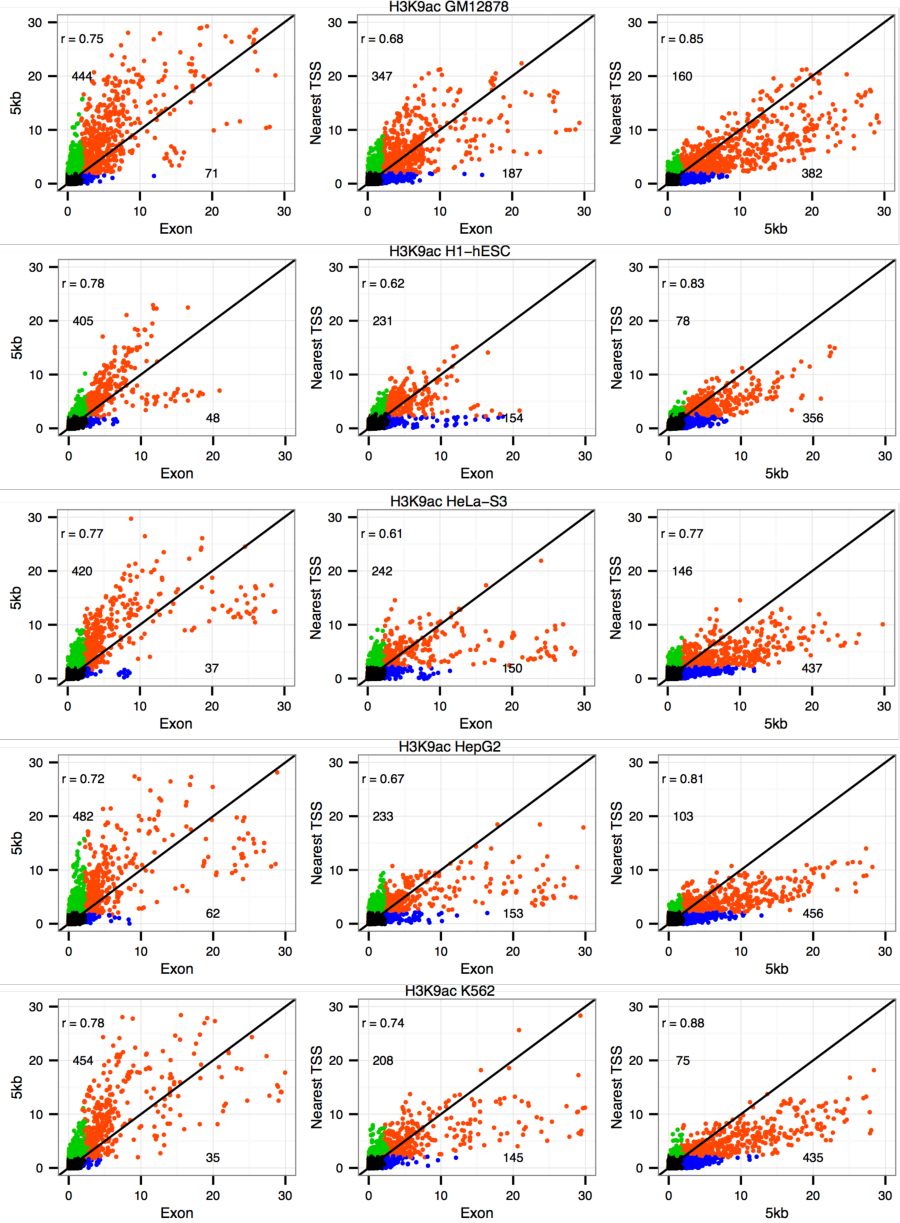
\includegraphics[width=0.8\textwidth]{chap2figs/figure2_8.pdf}
\caption[H3K9ac enrichment signal for different locus definitions.]
{
% Rackham requires the figure list title matches the first sentence, so repeat that sentence here
\textbf{H3K9ac enrichment signal for different locus definitions.} Enrichment signal (-log10 p-value) comparing nearest TSS, $\leq$ 5kb from TSS, and exons locus definitions for H3K9ac across 5 cell lines. Overall, $\leq$ 5kb and tends to perform better versus nearest TSS and versus exons. Note, for some gene sets exons clearly outperforms $\leq$ 5kb. This occurs specifically in embryonic stem cells and HeLa-S3 cells. Axes limits are constrained for visual clarity. Pearson correlation coefficient of all p-values (including those outside axis limits) is reported inset. Green points are unique enrichments ($\beta_1 > 0$ and $FDR < 0.05$) for the locus definition on the y-axis (number is inset), blue points are unique enrichments for the locus definitions on the x-axis (number is inset), orange points are enriched in both, and black in neither.
}
\label{chap2:fig:8}
\end{figure}

\newpage

\begin{figure}[ht!]
\centering
% manually adjust the width of the figure
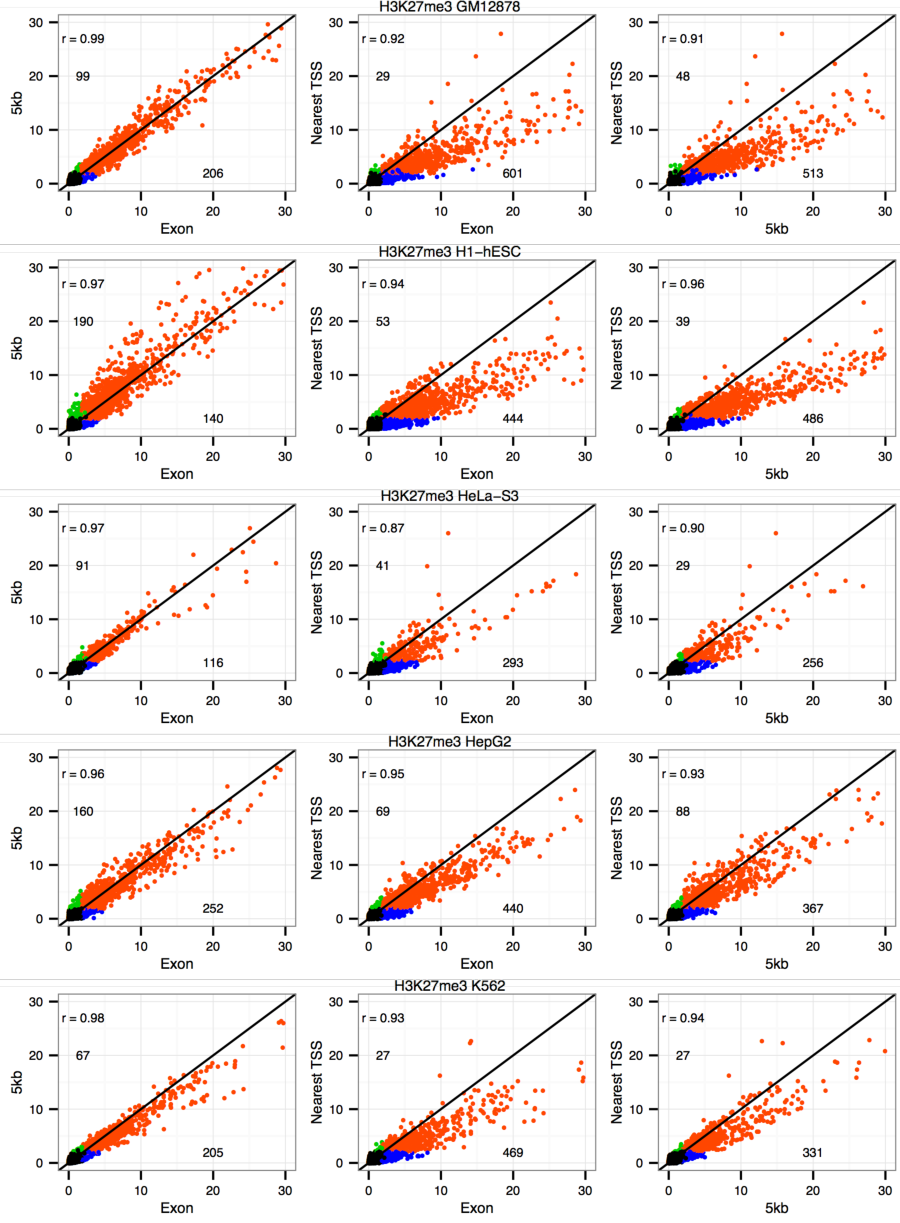
\includegraphics[width=0.8\textwidth]{chap2figs/figure2_9.pdf}
\caption[H3K27me3 enrichment signal for different locus definitions.]
{
% Rackham requires the figure list title matches the first sentence, so repeat that sentence here
\textbf{H3K27me3 enrichment signal for different locus definitions.} Enrichment signal (-log10 p-value) comparing nearest TSS, $\leq$ 5kb from TSS, and exons locus definitions for H3K27me3 across 5 cell lines. While both $\leq$ 5kb and exons perform better than nearest TSS, exons tends to perform slightly better than $\leq$ 5kb in all cell lines with the exception of H1-hESC. This could indicate a different regulatory regime for H3K27me3 in embryonic stem cells compared to the other, more differentiated, cell lines. Axes limits are constrained for visual clarity. Pearson correlation coefficient of all p-values (including those outside axis limits) is reported inset. Green points are unique enrichments ($\beta_1 > 0$ and $FDR < 0.05$) for the locus definition on the y-axis (number is inset), blue points are unique enrichments for the locus definitions on the x-axis (number is inset), orange points are enriched in both, and black in neither.
}
\label{chap2:fig:9}
\end{figure}

\newpage

\begin{figure}[ht!]
\centering
% manually adjust the width of the figure
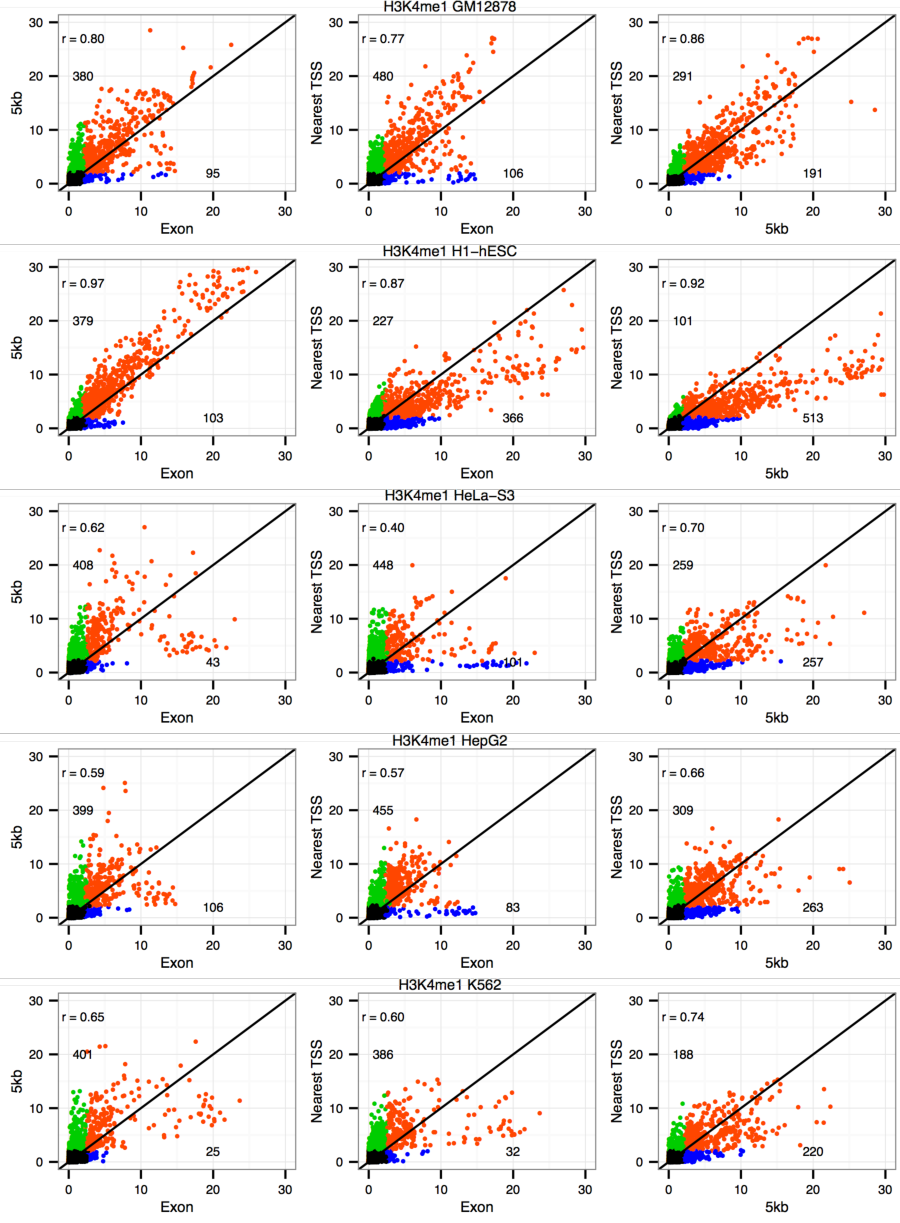
\includegraphics[width=0.8\textwidth]{chap2figs/figure2_10.pdf}
\caption[H3K4me1 enrichment signal for different locus definitions.]
{
% Rackham requires the figure list title matches the first sentence, so repeat that sentence here
\textbf{H3K4me1 enrichment signal for different locus definitions.} Enrichment signal (-log10 p-value) comparing nearest TSS, $\leq$ 5kb from TSS, and exons locus definitions for H3K4me1 across 5 cell lines. There is no clearly better performing locus definition across the cell lines. Nearest TSS performs better for GM12878 and HepG2, while $\leq$ 5kb performs better in H1-hESC, HeLa-S3, and K562. Recall, nearest TSS includes enhancer regions, whereas $\leq$ 5kb only includes proximal promoter regions. Consequently, the enrichment results may be a reflection of more long-range regulatory architecture in GM12878 and HepG2 versus more short-range architecture in the remaining cell lines. Axes limits are constrained for visual clarity. Pearson correlation coefficient of all p-values (including those outside axis limits) is reported inset. Green points are unique enrichments ($\beta_1 > 0$ and $FDR < 0.05$) for the locus definition on the y-axis (number is inset), blue points are unique enrichments for the locus definitions on the x-axis (number is inset), orange points are enriched in both, and black in neither.
}
\label{chap2:fig:10}
\end{figure}
